\begin{figure}[!ht]
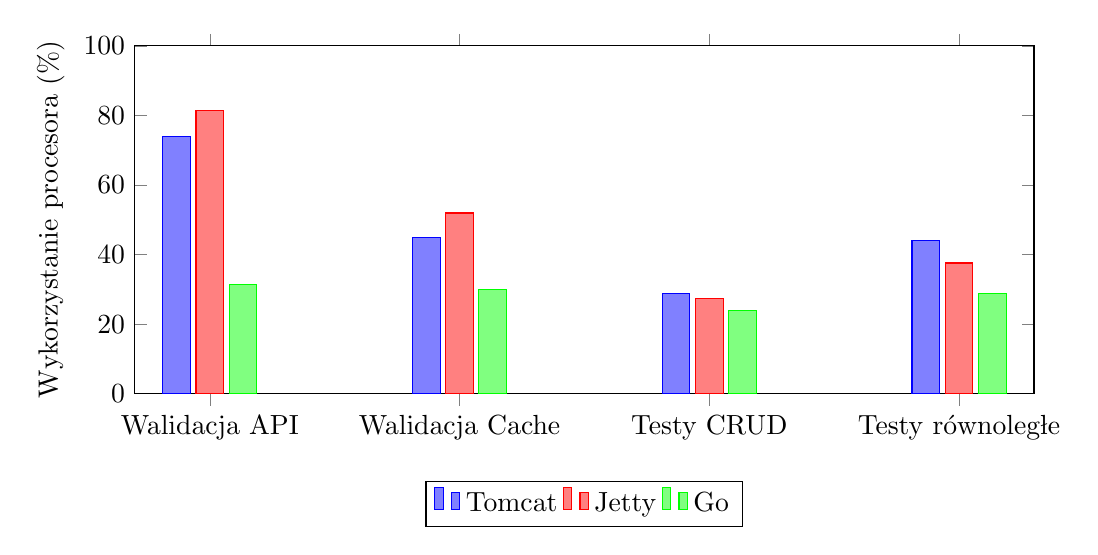
\begin{tikzpicture}
\begin{axis}[
    ybar,
    width=13cm,
    height=6cm,
    legend style={at={(0.5,-0.25)},
      anchor=north,legend columns=-1},
    ylabel={Wykorzystanie procesora (\%)},
    symbolic x coords={Walidacja API, Walidacja Cache, Testy CRUD, Testy równoległe},
    xtick=data,
    ymin=0, ymax=100
    ]

\addplot [blue, fill=blue!50!white] coordinates{ (Walidacja Cache,44.94) (Testy równoległe,43.92) (Walidacja API,74.01) (Testy CRUD,28.86) } ;
\addplot [red, fill=red!50!white] coordinates{ (Walidacja Cache,51.93) (Testy równoległe,37.57) (Walidacja API,81.33) (Testy CRUD,27.3) } ;
\addplot [green, fill=green!50!white] coordinates{ (Walidacja Cache,29.86) (Testy równoległe,28.85) (Walidacja API,31.35) (Testy CRUD,23.9) } ;

\legend{Tomcat,Jetty,Go}
\end{axis}
\end{tikzpicture}
\caption{Wykorzystanie procesowa przez aplikacje podczas testów z bazą danych wypełnioną danymi początkowymi - 100 klientów}
\label{fig:cpu_utilization_100_full}
\end{figure}

\begin{figure}[!ht]
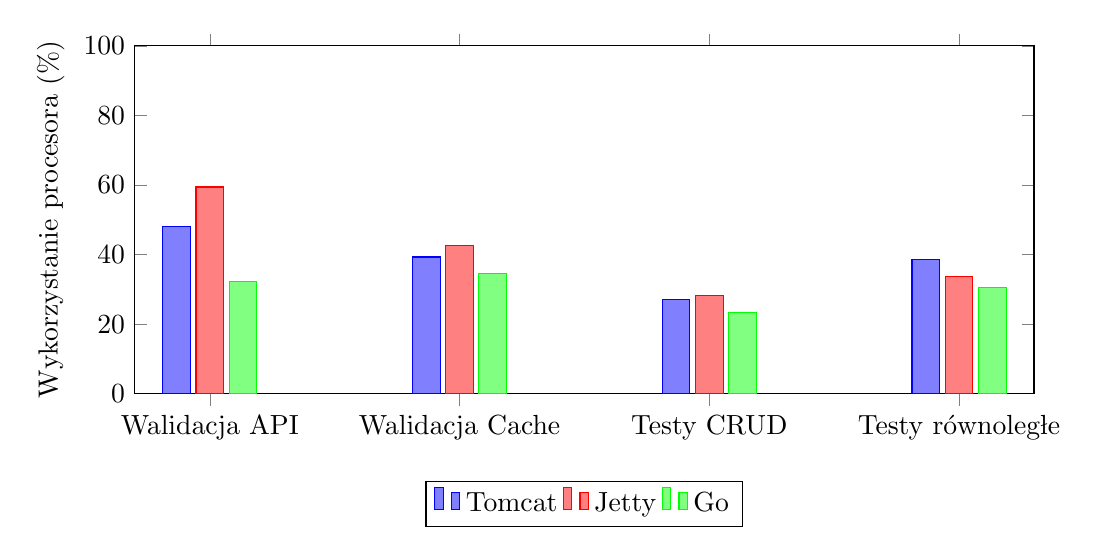
\begin{tikzpicture}
\begin{axis}[
    ybar,
    width=13cm,
    height=6cm,
    legend style={at={(0.5,-0.25)},
      anchor=north,legend columns=-1},
    ylabel={Wykorzystanie procesora (\%)},
    symbolic x coords={Walidacja API, Walidacja Cache, Testy CRUD, Testy równoległe},
    xtick=data,
    ymin=0, ymax=100
    ]

\addplot [blue, fill=blue!50!white] coordinates{ (Walidacja Cache,39.3) (Testy równoległe,38.52) (Walidacja API,47.96) (Testy CRUD,27.06) } ;
\addplot [red, fill=red!50!white] coordinates{ (Walidacja Cache,42.63) (Testy równoległe,33.75) (Walidacja API,59.42) (Testy CRUD,28.24) } ;
\addplot [green, fill=green!50!white] coordinates{ (Walidacja Cache,34.68) (Testy równoległe,30.64) (Walidacja API,32.38) (Testy CRUD,23.23) } ;

\legend{Tomcat,Jetty,Go}
\end{axis}
\end{tikzpicture}
\caption{Wykorzystanie procesowa przez aplikacje podczas testów z bazą danych wypełnioną danymi początkowymi - 250 klientów}
\label{fig:cpu_utilization_250_full}
\end{figure}